\documentclass{beamer}


\mode<presentation>
{
  \usetheme{CambridgeUS}
	\usecolortheme{beaver}
  % or ...

  \setbeamercovered{transparent}
  % or whatever (possibly just delete it)
}


\usepackage{xeCJK}
\usepackage{ulem}
\usepackage[english]{babel}
\usepackage[utf8]{inputenc}
\usepackage{times}
\usepackage[T1]{fontenc}
\usepackage{hyperref}
\usepackage{pifont}
\usepackage{biblatex}
\usepackage{bibentry}
\usepackage{verbatim}
\bibliography{cite}
\newcommand{\cmark}{\ding{51}}%
\newcommand{\xmark}{\ding{55}}%
\setCJKmainfont{WenQuanYi Micro Hei}
\renewcommand{\raggedright}{\leftskip=0pt \rightskip=0pt plus 0cm}
\raggedright

\let\oldfootnotesize\footnotesize
\renewcommand*{\footnotesize}{\oldfootnotesize\tiny}

\title[Big names in open source] 
{Big names in open source}
\subtitle{Eric Raymond}

\author[Zhilei Ren] 
{Zhilei Ren}

\institute[OSCAR Team] % (optional, but mostly needed)
{
\\
\includegraphics[width=0.2\textwidth]{../../utils/logo.jpg}\\
OSCAR Team, School of Software, 
Dalian University of Technology
}


\subject{Open Source}



\pgfdeclareimage[height=0.5cm]{university-logo}{../../utils/logo.jpg}
\logo{\pgfuseimage{university-logo}}



% Delete this, if you do not want the table of contents to pop up at
% the beginning of each subsection:
\AtBeginSubsection[]
{
  \begin{frame}<beamer>{Outline}
    \tableofcontents[currentsection,currentsubsection]
  \end{frame}
}


% If you wish to uncover everything in a step-wise fashion, uncomment
% the following command: 

%\beamerdefaultoverlayspecification{<+->}

\setbeamertemplate{section in toc}[circle]
\setbeamertemplate{items}[circle]
\setbeamertemplate{caption}[numbered]
\setbeamertemplate{bibliography item}{\insertbiblabel}
\setbeamertemplate{bibliography entry title}{}
\setbeamertemplate{bibliography entry journal}{}

\begin{document}

\begin{frame}
  \titlepage
\end{frame}

%\begin{frame}{Outline}
%  \tableofcontents[currentsection,currentsubsection, 
%    hideothersubsections, 
%    sectionstyle=show,
%]
%\end{frame}

\AtBeginSection[]
{
 \begin{frame}<beamer>
 \frametitle{Outline}
 \tableofcontents[currentsection]
 \end{frame}
}

% \begin{frame}[t]{How To Ask Questions The Smart Way}
% 
%   %  http://www.catb.org/~esr/faqs/smart-questions.html
%   %  https://github.com/ryanhanwu/How-To-Ask-Questions-The-Smart-Way/blob/master/README-zh_CN.md
%     
% \end{frame}

\begin{frame}[c]{I'm with those guys}
    \centering
    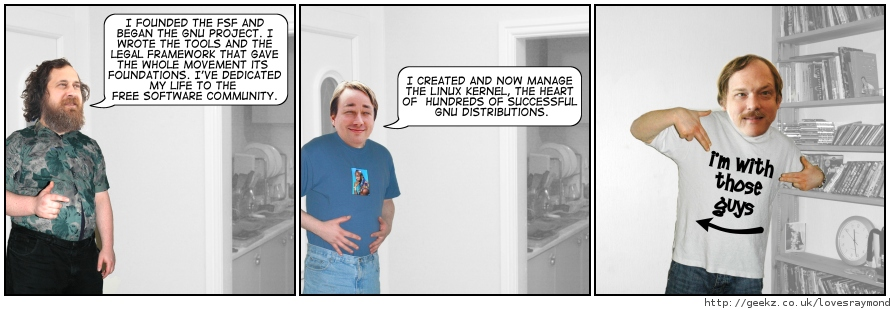
\includegraphics[width=.7\textwidth]{../../part1/lecture1/eric.jpg}    
\end{frame}

\begin{frame}[t]{The new hacker's dictionary}
    \centering
    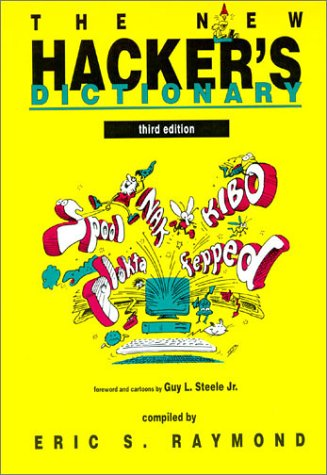
\includegraphics[width=.3\textwidth]{jargon-file.jpg} 

    a.k.a The jargon file
\end{frame}

\begin{frame}[t]{The new hacker's dictionary\footnote{\url{https://en.wikipedia.org/wiki/Eric_S._Raymond}}}
Raymond began his programming career writing proprietary software, between 1980 and 1985. In 1990, noting that the Jargon File had not been maintained since about 1983, he adopted it; he currently has a third edition in print. Paul Dourish maintains an archived original version of the Jargon File, because, he says, Raymond's updates "essentially destroyed what held it together." \footnote{\url{http://www.dourish.com/goodies/jargon.html}}
\end{frame}

\begin{frame}[t]{How To Ask Questions The Smart Way\footnote{\url{https://github.com/FredWe/How-To-Ask-Questions-The-Smart-Way}}}
    \begin{enumerate}
      \item 声明
      \item 简介
      \item 在提问之前
      \item 当你提问时
      \item 如何解读答案
      \item 如何避免扮演失败者
      \item 不该问的问题
      \item 好问题与蠢问题
      \item 如果得不到回答
      \item 如何更好地回答问题
      \item 相关资源
      \item 鸣谢
    \end{enumerate}
\end{frame}

\begin{frame}[t]{The Cathedral and the Bazaar}
    \centering
    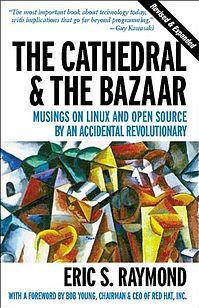
\includegraphics[width=.3\textwidth]{Cathedral-and-the-Bazaar-book-cover.jpg} 
\end{frame}

\begin{frame}[t]{The Cathedral and the Bazaar}
    
    最初,有一种人叫“真程序员”( Real Programmer )。他们并不这样自称,也不自称为黑客或者别的什么。据他们中的一位回忆,“真程序员”这个称呼是在上世纪 80 年代以后才出现的。自 1945 年以来,计算机技术吸引了世界上最睿智和最有创意的人,从 Eckert 和 Mauchly 发明的第一台 ENIAC 开始,就有一批编程爱好者,并或多或少伴随着一种他们自己能意识到的技术文化,他们编软件和玩软件只是出于乐趣。

    “真程序员”通常具备工程学和物理学背景,并常常是业余无线电爱好者。他们穿着白色袜子、涤纶衬衫,打着领带,带着厚厚的眼镜,使用机器语言、汇编语言、 FORTRAN 或者其他一些已经被人们遗忘了的古老的编程语言。

    “真程序员”文化和批处理计算(尤其是批处理技术)密切相关,随着交互式计算、大学和网络的兴起,“真程序员”文化逐渐衰落,另一个工程师文化诞生并最终演化成今天的开源黑客文化。
\end{frame}

\begin{frame}[t]{Real Programmers\footnote{\url{https://www.xkcd.com/378/}}}

    \centering
    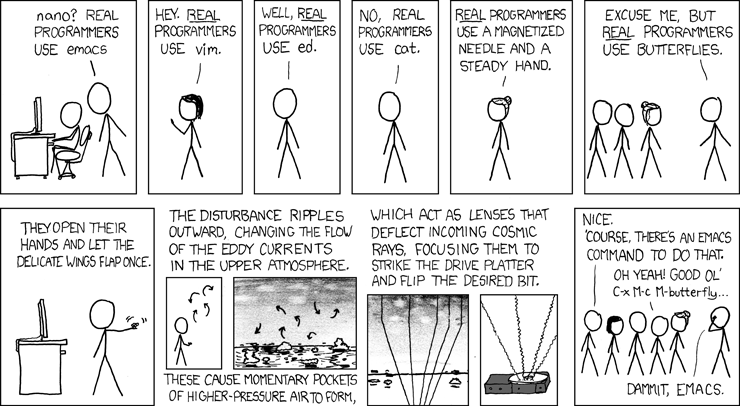
\includegraphics[width=.7\textwidth]{real_programmers.png}
\end{frame}

\begin{frame}[t]{Aunt Tillie}
    \begin{enumerate}
        \item Aunt Tillie test: The archetypal non-technical user, one's elderly and scatterbrained maiden aunt. Invoked in discussions of usability for people who are not hackers and geeks; one sees references to the ``Aunt Tillie test''
        \item The term was invented by Eric Raymond, who added it to the Jargon File despite being the only person who used it.
        \item The irony, as pointed out by John Gruber regarding the linux-kernel post in which Aunt Tillie was first invoked: ``It wasn't [Aunt Tillie] who couldn't connect to a shared printer. It was Raymond himself who couldn't figure it out.''\footnote{\url{https://daringfireball.net/2004/04/spray_on_usability}}
    \end{enumerate}
    
\end{frame}
\begin{frame}[t]{Aunt Tillie}
    \centering
    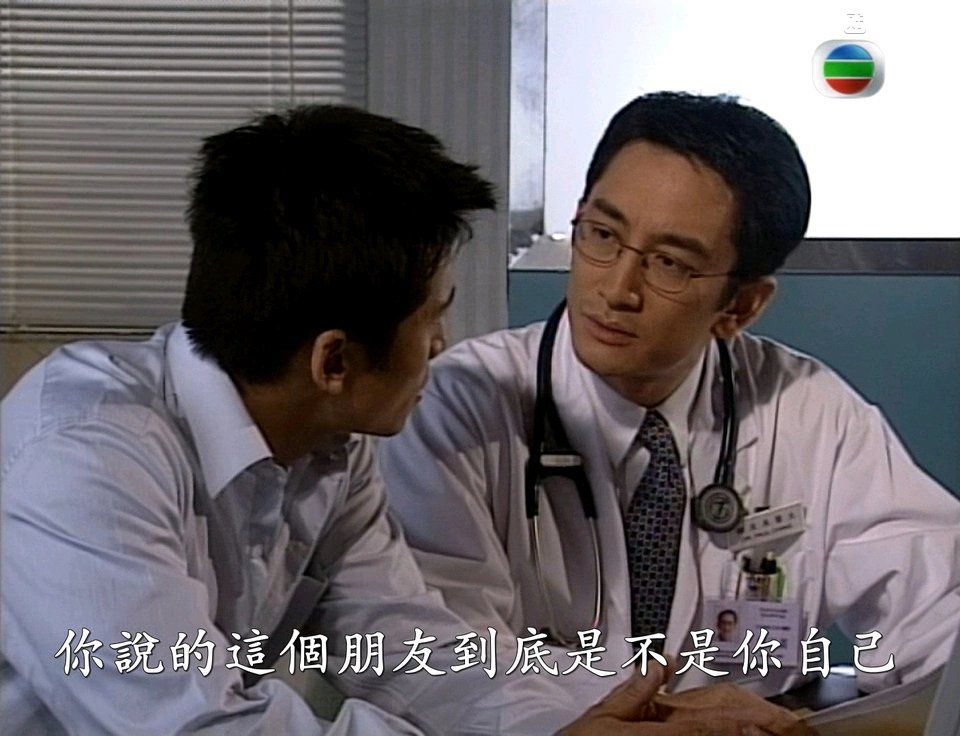
\includegraphics[width=.5\textwidth]{friends.png}

    你说的这个\sout{朋友}Aunt Tillie到底是不是你自己
    
\end{frame}

\end{document}

